% \begin{tikzpicture}
\node at (0,0) {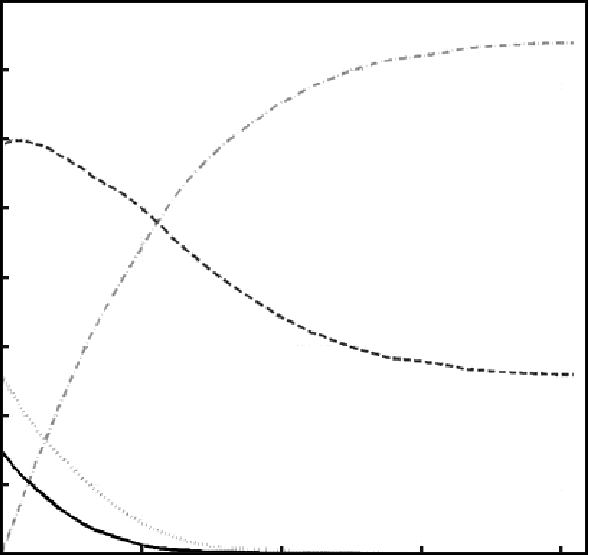
\includegraphics[width=6cm]{img/chap5/brill2_refait}};

\draw[legende] (-1.1,-1.1) rectangle (2.9,-2.7);

\draw (-0.4,-1.3) node[anchor=west, font=\footnotesize] {fausse égalité};
\draw (-0.4,-1.7) node[anchor=west, font=\footnotesize] {fausse différenciation};
\draw (-0.4,-2.1) node[anchor=west, font=\footnotesize] {faux ordonnancement};
\draw (-0.4,-2.5) node[anchor=west, font=\footnotesize] {décision correcte};

\draw[very thick, help lines, densely dashed] (-1,-1.3) -- (-0.4,-1.3);
\draw[thick, help lines, densely dotted] (-1,-1.7) -- (-0.4,-1.7);
\draw[very thick] (-1,-2.1) -- (-0.4,-2.1);
\draw[very thick, densely dashed] (-1,-2.55) -- (-0.4,-2.55);

\node[below=0.3cm,rotate=90] at (-4,0.5) {Proportions};
\node[anchor=east] at (-2.9,-2.8) {0};
\node[anchor=east] at (-2.9,-2.1) {0,1};
\node[anchor=east] at (-2.9,-1.4) {0,2};
\node[anchor=east] at (-2.9,-0.7) {0,3};
\node[anchor=east] at (-2.9,0) {0,4};
\node[anchor=east] at (-2.9,0.7) {0,5};
\node[anchor=east] at (-2.9,1.4) {0,6};
\node[anchor=east] at (-2.9,2.1) {0,7};
\node[anchor=east] at (-2.9,2.8) {0,8};

\node at (0,-3.5) {$\Delta \mathit{OVQM}$};
\node[anchor=north] at (-3,-2.8) {0};
\node[anchor=north] at (-1.6,-2.8) {0,1};
\node[anchor=north] at (-0.1,-2.8) {0,2};
\node[anchor=north] at (1.3,-2.8) {0,3};
\node[anchor=north] at (2.7,-2.8) {0,4};


% \end{tikzpicture}